\documentclass[10pt]{article}
\usepackage[pdftex]{graphicx}
\usepackage{amsmath,amssymb}
\usepackage{dirtytalk}
\usepackage{xcolor}
\usepackage{hyperref}
\hypersetup{
    colorlinks,
    linkcolor={red!50!black},
    citecolor={blue!50!black},
    urlcolor={blue!80!black}
}
\usepackage[skip=10pt plus1pt, indent=40pt]{parskip}
\usepackage{../common_styles/csagh}


\begin{document}
\begin{opening}
  \title{Multiple linear regression with Python}
  \author[Universidad Autónoma de Nuevo León, San Nicolás de los Garza, aldo.hernandezt@uanl.edu.mx]{Aldo Hernández}

  \keywords{...}
  \begin{abstract}
    Multiple linear regression is a very common model used in machine learning, although it may not be the best option in the vast majority of cases. Nonetheless, it remains fairly useful when we need to determine a tendency in a large dataset based on certain characteristics (or labels) of interest. This document serves as an introduction to multiple linear regression and its applications with the programming language Python. In order to do this we will explore definitions, mathematical formulas, and pieces of code to make predictions on a dataset. Conclusions indicate that even though the model is not trustworthy, we can see a tendency in our set of data given one or two labels that may indicate a relationship between them and our outcome of interest. This suggests that for a small dataset where underfitting is very common, multiple linear regression should be used only for finding tendencies, instead of making our predictions on this type of model.
  \end{abstract}

  \keywords{multiple linear regression, python, model, tendency, machine learning}
\end{opening}

\section{Introduction}
Multiple linear regression is a vastly used algorithm in statistics and machine learning to make predictions and show tendencies given a certain dataset. This algorithm \textit{finds} a linear function that indicates the tendency ---usually thought as a straight line in two dimensions--- and makes predictions from it. \cite{aprendeML} \par
Said function is represented as it follows
\begin{equation*}
    y = \beta_{0} + \beta_{1}x_{1} + \beta_{2}x_{2} + \dots + \beta_{n}x_{n}
\end{equation*}
where $\beta_{i}$ is the coefficient ---also known as weight--- for the $i$-th independent variable $x$ that represents a characteristic --or label-- that we are analyzing in the model. \par
If the reader is already familiarized with some concepts of machine learning, it is easy to see why linear regression is considered as a \textbf{supervised algorithm}. We should remember that the task of supervised learning is:
\vspace{5pt}

\say{Given a training set of N example input-output pairs \\ 
\hspace*{60pt} ($x_{1}, y_{1}$), ($x_{2}, y_{2}$), \dots ($x_{N}, y_{N}$) \\
\hspace*{20pt}where each $y_{i}$ was generated by an unknown function $y = f(x)$, discover a \hspace*{20pt}function $h$ that approximates the true function $f$.} \cite{ai}
\vspace{5pt}

So since the dataset is already labeled with information we want to take into account to predict a certain outcome, and we have our $N$ input-output pairs given our specific tags. \par
It remains obvious that this definition can be applied to multiple linear regression if we change the training set from pairs to an $n$-tuple with $n-1$ tags and one output.

\newpage

\section{Methodology}
\subsection{Before typing code}
Before we start the activity, we must download the following \href{http://www.aprendemachinelearning.com/articulos_ml/}{.csv file} \cite{aprendeML} to use the same dataset. Also, we have to import the following Python packages:
\begin{itemize}
  \item Numpy
  \item Pandas
  \item Matplotlib
  \item Scikit-learn
\end{itemize}
After doing this, we are ready to import all of the needed packages to our Python main file: \par
\begin{figure}[h]
  \centering
  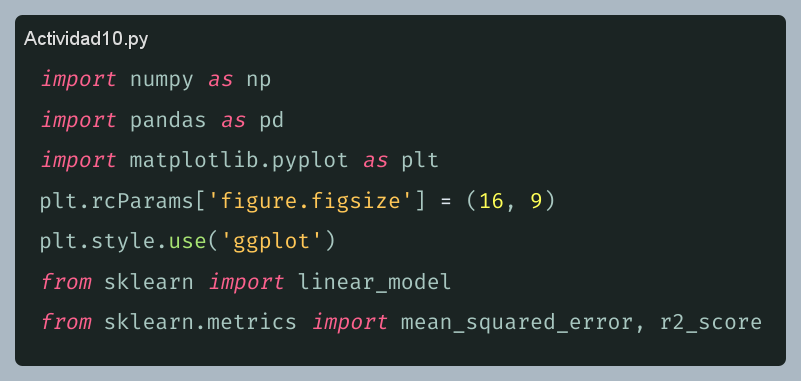
\includegraphics[width=90mm]{images/2025-03-25-09-38-02}
  \caption{Necessary imports and starting configurations for the activity.}
\end{figure}
As the reader can see, we also made some specific configuration for the program plots, such as size (in line 4) and style (in line 5); this may be changed according to the reader's preferences.

\subsection{Data processing}
Next, we will read the data from the .csv file using pandas to transform it into a dataframe. This is necessary since it will help us to easily remove all the columns that we will not use for the analysis, as shown in the figure: \par
\begin{figure}[h]
  \centering
  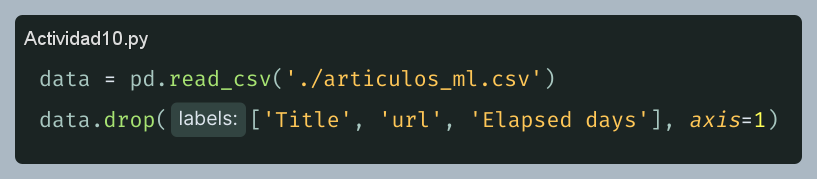
\includegraphics[width=90mm]{images/2025-03-25-10-23-22}
  \caption{Reading the data and removing unimportant columns from the dataframe.}
\end{figure}

\subsection{Filtering data}
Now that we have all of our essential data, we need to filter it in order to remove random anomalies in the dataset. In order to do this, we will take a look into the dataset information with the data.describe() method, but only to our two main columns:

\begin{table}[!ht]
  \centering
  \caption{Column information}
  \label{col_info}
    \begin{tabular}{|c|c|c|}
      \hline
       & Word count & \# Shares \\
      \hline
      Count & 161 & 161 \\
      \hline
      Mean & 1808.26 & 27948.348 \\
      \hline
      Std & 1141.919 & 43408.007 \\
      \hline
    \end{tabular}
\end{table}

As we can see in table \ref{col_info}, there are no null values in the columns, and our values are not very concentrated. Since we can't do really much with this information, we will graph a histogram to see where our data is really concentrated using the hist() method right after dropping the unnecessary columns: \par

\begin{figure}[h]
  \centering
  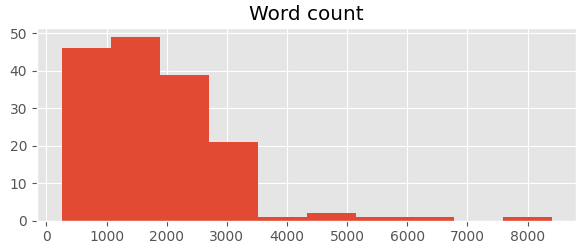
\includegraphics[width=55mm]{images/2025-03-25-10-49-04}
  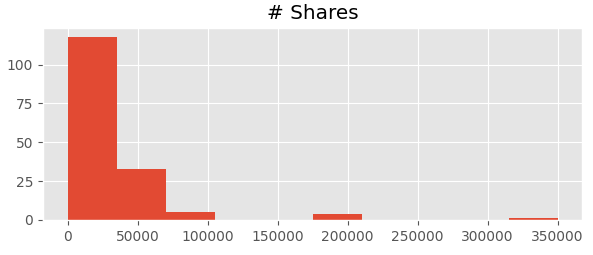
\includegraphics[width=55mm]{images/2025-03-25-10-49-28}
  \caption{Data concentration histogram of the Word count and \# Shares columns.}
\end{figure}

Thanks to these graphics, we can now filter the data to remove anomalies. To do so, we will simply remove all data with more than 3500 words and data with more than 80000 shares with the following code: \par

\begin{figure}[h]
  \centering
  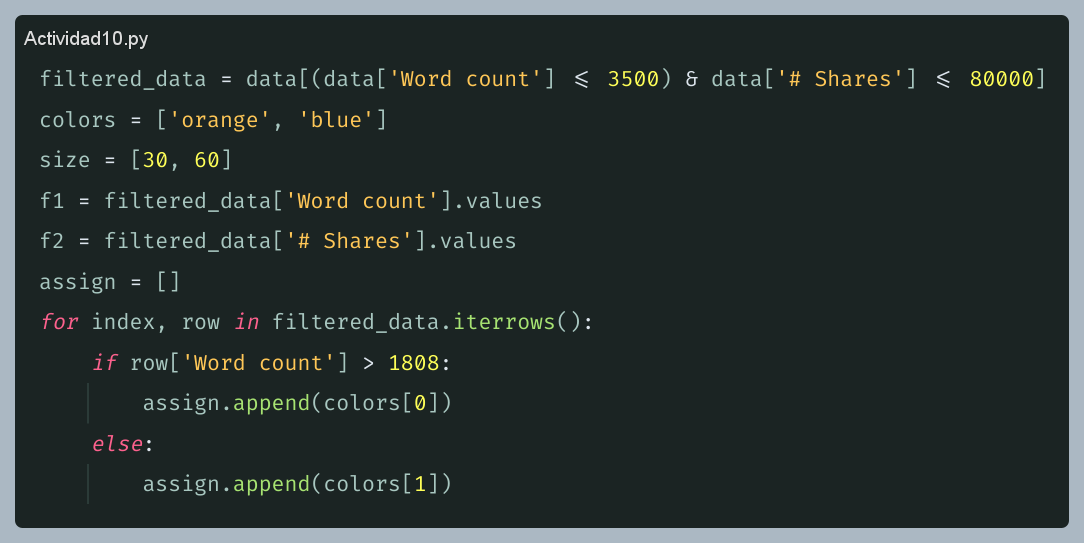
\includegraphics[width=90mm]{images/2025-03-25-11-02-42}
  \caption{Data filtering from the original dataset}
\end{figure}

We also colored data with orange if they are over the word count mean, or blue otherwise.

\subsection{Creating a new dataframe}
To create our multiple regression model, we will have to create a new dataframe with the columns that we will use as inputs. In this case, we will keep word count, but the other column will be the sum of links, comments, and images or videos. \par

\begin{figure}[h]
  \centering
  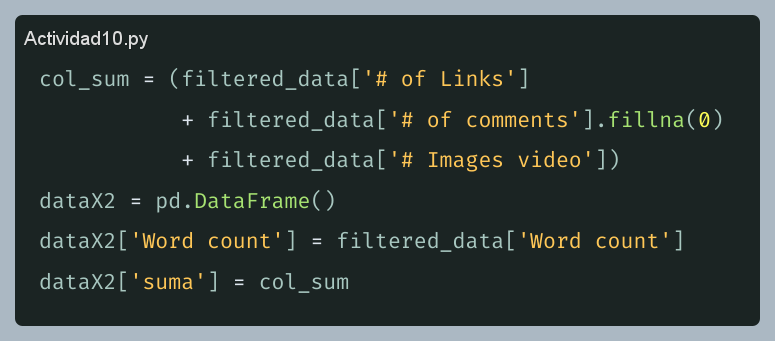
\includegraphics[width=90mm]{images/2025-03-25-11-12-20}
  \caption{Creating a new dataframe with $x_{1}$ and $x_{2}$ as our input columns.}
\end{figure}

We then create our training set as a NumPy array for $x$, $y$, and $z$, which are our 3-tuples $(x_{1}, y_{1}, z_{1})$

\begin{figure}[h]
  \centering
  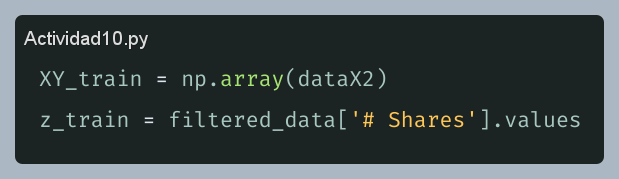
\includegraphics[width=90mm]{images/2025-03-25-11-16-52}
  \caption{Training set for the multiple linear regression model.}
\end{figure}

Finally, we create our model and fit it to the training data.

\begin{figure}[h]
  \centering
  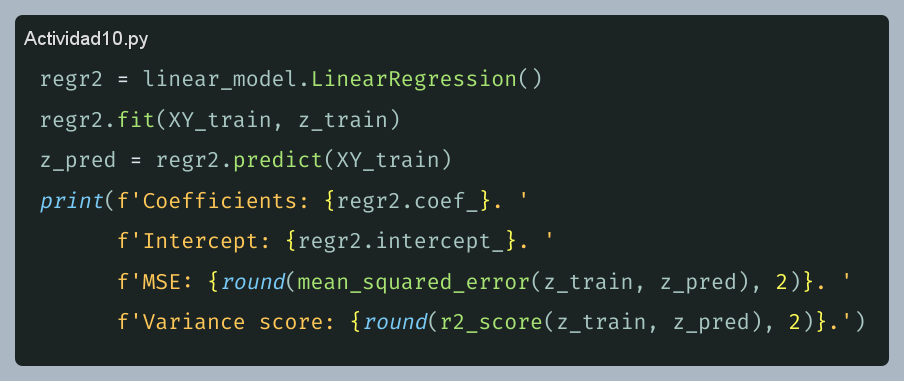
\includegraphics[width=80mm]{images/2025-03-25-11-24-07}
  \caption{Multiple linear regression model.}
\end{figure}

The reader may notice that we also print the coefficients $\left\{\beta_{0}, \beta_{1}, \beta_{2}\right\}$ of the linear function used for the model and some metrics to check the effectiveness of the model. These metrics are the \textit{Mean Squared Error}, and the \textit{Variance score}, where in ideal cases the MSE should be low and the variance score near one, which is not the case.

\subsection{Making a 3D graph with Matplotlib.pyplot}
Finally, we create a 3D plot using our new dataframe. We will start by creating a meshgrid where all of our $x$ and $y$ data will be distributed, and then make all of our plot values of a certain color (blue if from original set, red if it comes from a prediction using the training set). \par

\begin{figure}[h]
  \centering
  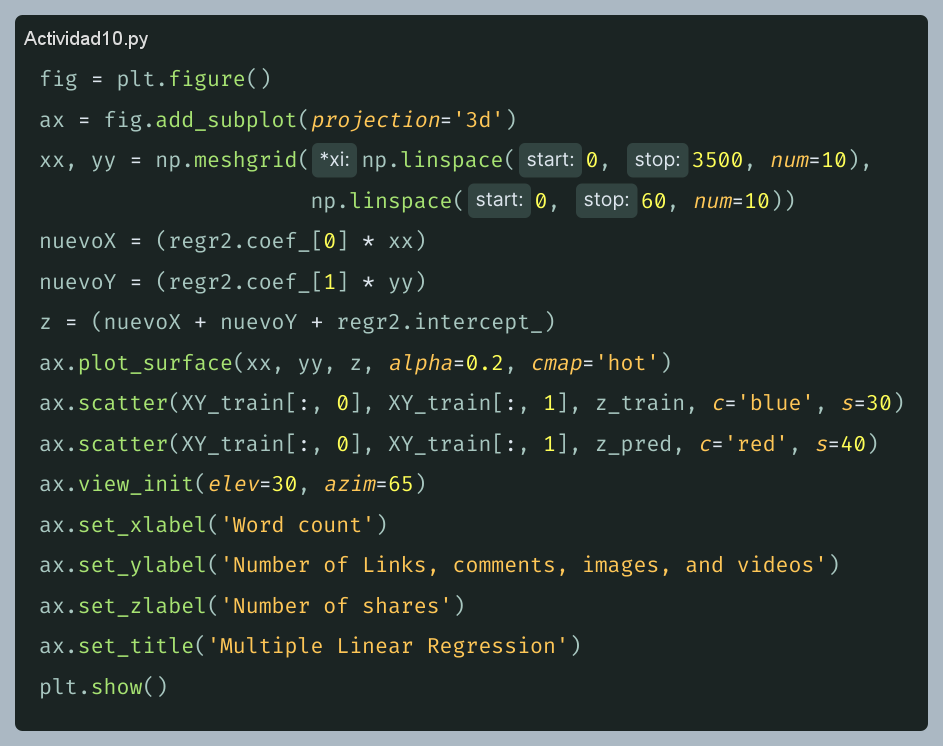
\includegraphics[width=90mm]{images/2025-03-25-11-39-30}
  \caption{Creating the 3D plot.}
\end{figure}

\newpage

The reader may wonder why the plot contains a big 2D plane, and it is as simple as that a line in 2D is a plane in 3D. With that stated, it is quite easy to visualize that said plane is our model, represented by the linear function
\begin{equation*}
  z = 21140.97 + 0.493x + 289.3253y
\end{equation*}

\begin{figure}[h]
  \centering
  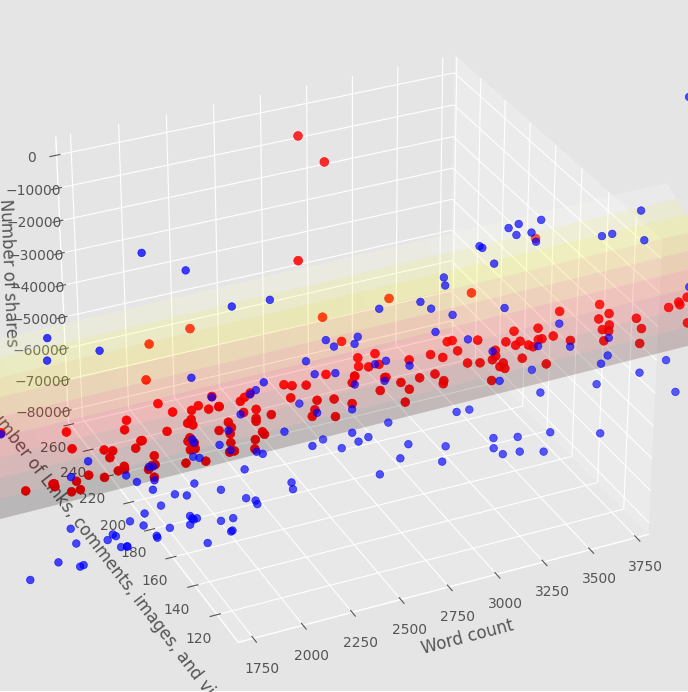
\includegraphics[width=90mm]{images/2025-03-25-11-43-19}
  \caption{Final 3D plot.}
\end{figure}

\section{Results}
Even though our model is not trustworthy, we can still make some predictions with it. For example, let's suppose we have an article with 2000 words, 10 links, 4 comments, and 6 images, according to our model, we would have around 27913 shares:
\begin{equation*}
  z = 21140.97 + 0.493(2000) + 289.3253(10+4+6) \approx 27913
\end{equation*}

\section{Conclusions}
Guided by the used metrics, it turned out our model was not trustworthy given the dataset. Although it seems like a failure, the model helped to find a tendency: the more words, links, comments, and images an article has, the more shares it will have. Of course it is not as simple as that, but given these inputs, the model suggests that this is true. We could prove it by reducing dimensions using an algorithm like Principal Component Analysis, but that is out of the purpose of this article. \par
Therefore, we conclude that the model is not suitable for small and dispersed datasets since it will probably lead to an underfitted model that will make bad predictions, but it remains useful to find a tendency early on during a larger investigation.

\bibliographystyle{../common_styles/cs-agh}
\bibliography{act10_bibliography}

\end{document}